\documentclass[14pt, a4paper]{SCWorks}

\usepackage[T2A]{fontenc}
\usepackage[utf8]{inputenc}
\usepackage[english, russian]{babel}

\usepackage{amsmath, amsfonts, amssymb}

\usepackage{graphicx}
\usepackage{float}

\usepackage{minted}

\setminted[python]{
    fontsize=\small,
    breaklines=true,
    style=bw,
    linenos,
    frame=lines,
    framesep=2mm,
    baselinestretch=1.2
}

\renewcommand\theFancyVerbLine{\small\arabic{FancyVerbLine}}

\title{Алгоритм шифрования RSA: математические основы и программная реализация}
\author{Миронов Г. О.}
\date{\today}

\course{1} 
\group{151} 
\napravlenie{09.03.01 Программная Инженерия} 
\department{факультета КНиИТ} 

\chair{Математической кибернетики и компьютерных наук} 
\chtitle{доцент, к.ф.-м.н.} 
\chname{Иванов И. И.} 
\satitle{доцент, к.ф.-м.н.} 
\saname{Петров П. П.} 

\begin{document}

\maketitle

\tableofcontents
\newpage

\section{Введение}

В современном мире защита информации играет ключевую роль. Алгоритм RSA "--- один из самых известных алгоритмов асимметричного шифрования, который был предложен в 1977~году Рональдом Ривестом, Ади Шамиром и Леонардом Адлеманом~\cite{rsa_original}.

Суть асимметричного шифрования заключается в использовании пары ключей: открытого ключа \texttt{public\_key} для зашифрования данных и закрытого ключа \texttt{private\_key} для их расшифрования. В данной работе будут рассмотрены математические принципы, лежащие в основе данного алгоритма, а также приведена его программная реализация на языке Python~\cite{python_docs}.

\section{Математические основы RSA}

Безопасность алгоритма RSA базируется на вычислительной сложности задачи факторизации больших целых чисел. Генерация ключей начинается с выбора двух различных простых чисел \texttt{p} и \texttt{q}. Первым шагом вычисляется их произведение:
$n = p \cdot q$

Число \texttt{n} называется модулем и используется как часть как открытого, так и закрытого ключей. Далее вычисляется функция Эйлера от числа \texttt{n}:
\begin{equation}
\label{eq:euler}
\varphi(n) = (p - 1)(q - 1)
\end{equation}

После этого выбирается целое число \texttt{e}, такое что $1 < e < \varphi(n)$, причем \texttt{e} и $\varphi(n)$ должны быть взаимно простыми. Число \texttt{e} становится открытой экспонентой. Затем вычисляется число \texttt{d}, называемое секретной экспонентой, которое удовлетворяет следующему условию:
\begin{equation}
\label{eq:secret_d}
d \cdot e \equiv 1 \pmod{\varphi(n)}
\end{equation}

Процессы шифрования исходного сообщения \texttt{m} и расшифрования полученного шифротекста \texttt{c} можно описать с помощью следующих математических выражений:
\begin{align}
c &\equiv m^e \pmod{n} \label{eq:encrypt} \\
m &\equiv c^d \pmod{n} \label{eq:decrypt}
\end{align}

Как видно из уравнений~\ref{eq:encrypt} и~\ref{eq:decrypt}, а также свойства функции Эйлера~\ref{eq:euler}, процесс восстановления данных требует наличия секретного ключа.

\section{Программная реализация и тестирование}

Для визуализации работы алгоритма рассмотрим общую схему обмена ключами, представленную на рисунке~\ref{fig:keys_exchange}.

\begin{figure}[H]
\centering
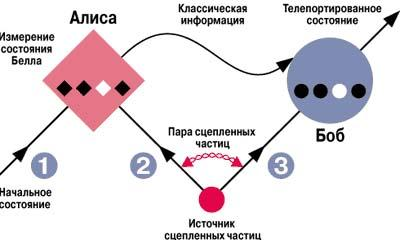
\includegraphics[scale=0.8]{img/keys.png}
\caption{Схема обмена асимметричными ключами}
\label{fig:keys_exchange}
\end{figure}

В процессе передачи информации данные преобразуются согласно схеме шифрования, проиллюстрированной на рисунке~\ref{fig:encryption_schema}.

\begin{figure}[H]
\centering
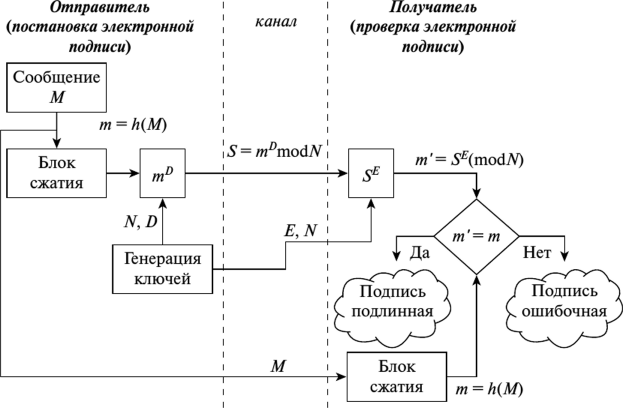
\includegraphics[scale=0.8]{img/schema.png}
\caption{Схема процесса шифрования и расшифрования RSA}
\label{fig:encryption_schema}
\end{figure}

Программная реализация алгоритма генерации ключей, шифрования и расшифрования на языке программирования Python~\cite{python_docs} вынесена в отдельный файл. Исходный код представлен ниже.

\inputminted{python}{src/rsa.py}

Для проверки корректности работы реализованного алгоритма было проведено тестирование на наборе входных данных. Результаты тестирования для различных исходных сообщений \texttt{m} и параметров ключей приведены в таблице~\ref{tab:test_results}.

\begin{table}[H]
\centering
\caption{Результаты тестирования алгоритма RSA}
\label{tab:test_results}
\begin{tabular}{|c|c|c|c|c|}
\hline
$p$ & $q$ & Исходное сообщение $m$ & Шифротекст $c$ & Расшифрованное сообщение \\
\hline
61 & 53 & 65 & 2790 & 65 \\
17 & 19 & 88 & 192 & 88 \\
23 & 29 & 42 & 101 & 42 \\
\hline
\end{tabular}
\end{table}

\section{Заключение}

В ходе выполнения работы были изучены основные математические принципы работы алгоритма асимметричного шифрования RSA~\cite{rsa_original}. Были рассмотрены процессы генерации ключей, шифрования и расшифрования сообщений. Программная реализация на языке Python продемонстрировала практическую применимость теоретических выкладок. Результаты тестирования, представленные в таблице~\ref{tab:test_results}, подтверждают корректность работы алгоритма.


\newpage
\bibliographystyle{gost780uv}
\bibliography{thesis}

\end{document}